%!TEX ROOT = thesis.tex
\chapter{Framework Overview}

\section{Introduction}
In order to tackle the issues identified through the research questions and literature review, the theoretical framework is laid as to provide a conceptual schema on how to break the rather huge and intricate challenge into multiple bite sized puzzles. First, some reoccurring key concepts used throughout this work is discussed in Section \ref{section:keyconcepts}. This is then followed by the overview of the proposed framework used in this work is described in Section \ref{section:framework}. Next, the description of the dataset used is described in Section \ref{section:dataset_used} and finally, this chapter concludes with the experimental methodology applied in this work to obtain the published results (see Section \ref{sec:expmethodology}). 

\section{Key Concepts}
\label{section:keyconcepts}
Before diving deeper into the nitty-gritty of the proposed framework, fundamental understanding towards the key concepts used in this work is discussed. As this work covers a rather broad spectrum of different concepts, a general understanding towards these key concepts would provide some degree of clarity towards the topic at hand. This section briefly describes the fundamental of the following key concepts: i) Quantization, ii) Distance Measure \& iii) Color Model. 


\subsection{Quantization}

The use of quantization in the mathematical and digital signal processing field is not a new concept. However, digital signal processors are limited by natural boundaries such as hardware limitations, and are only able to compute and perform arithmetic operations within a limited range \cite{spors_2018}. The use of quantization refers to the process of mapping and projecting a set of large values which are often continuous or analog in nature into a set of discrete and finite values. 

\begin{figure}[hbt!]\centering
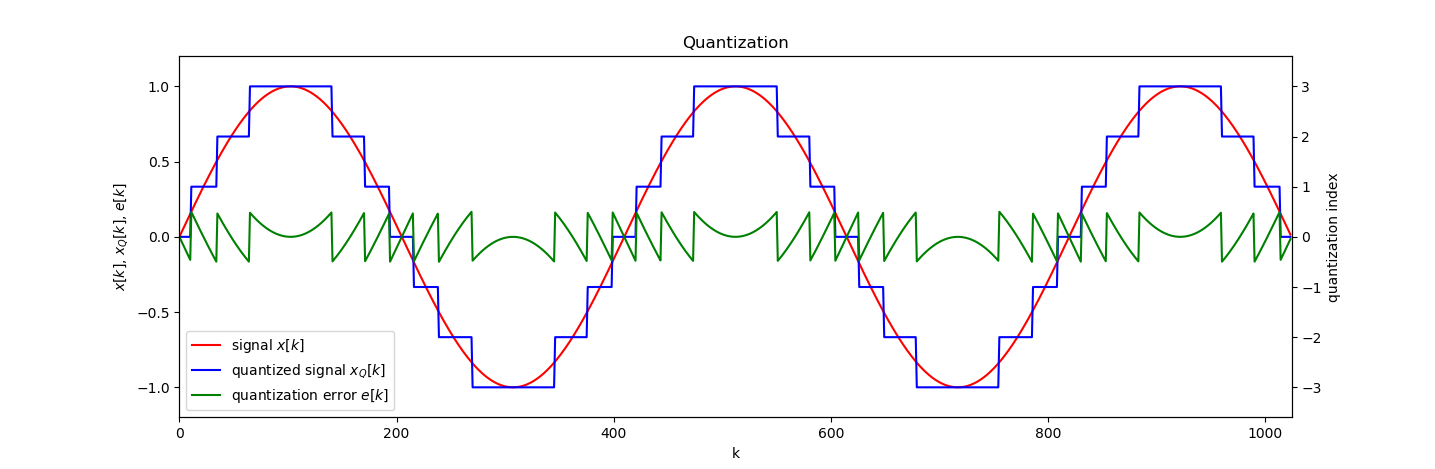
\includegraphics[width=\textwidth]{image/general/quantization.png}
\caption{Quantization}
\end{figure}


The use of quantization enables reduction in memory usage (compression) as well as the reduction of computational cost, hence, leading to faster processing speed. However, since quantization is a many-to-few mapping operation, hence, the operation is considered irreversible without prior knowledge of the loss. Nevertheless, the output discrete signal can closely resemble the continuous input signal depending on the number of quantization level used.

In the proposed method, the quantization technique was extended further into a three dimensional space where the 3D space is quantized into a set of discrete and finite values to ease the calculation and manipulation of data in the both the video data as well as the color space. 

\begin{equation}\centering
\label{eq:quantization}
x_Q[k] = g( \mspace{3mu}\lfloor \mspace{3mu}f(x[k]) \mspace{3mu}\rfloor\mspace{3mu})
\end{equation} 

\vspace{-3em}


\begin{equation}\centering
\label{eq:quantizationerror}
e[k] = x_Q[k] - x[k]
\end{equation}


In order to expound on the quantization process, a mathematical model of this process can be formulated as such. Consider a continuous signal $x[k]$ whose quantized signal, $x_Q[k]$, is desired, Equation \ref{eq:quantization}. The functions $f (\mspace{3mu} \cdot  \mspace{3mu})$ \& $g (\mspace{3mu} \cdot  \mspace{3mu})$ can be thought of as a real-value mapping function while the $\lfloor \mspace{3mu} \cdot  \mspace{3mu} \rfloor$ represents a rounding function. As previously mention, this process is considered irreversible with prior knowledge of the loss, in this case, the quantization error, $e[k]$, can be computed as Equation \ref{eq:quantizationerror}. 

\subsection{Distance Measure}
\label{section:distancemeasures}

The use of distance metrics is another recurring key concept in the proposed methods. While distance measure is commonly used in computer science as well as the mathematics field, there are numerous metrics suggested by different authors which are applicable and useful in different scenarios. 

To further accentuate on the concept of distance measure in this work, a simple example of how distance metrics can be applied in the proposed method is illustrated using Figure \ref{fig:distanceMeasure} with two plotted lines. In order to simplify the research problem, these lines can be thought of as vehicle trajectories captured over time, and flatten unto a 2D plot. Using the available data, the distance between two trajectories can be measured and used to signify the dissimilarity between them. This distance measure can also be used to identify trajectories with high resemblance. 

However, as different distance measure metrics are suitable for different scenarios, a good distance measure is an essential for comparing a significantly extensive set of vehicle trajectories during the retrieval process of a car park scene. This concept of distance measure was further extended into a multi-dimensional space such as the colors space, where the similarity between two or more colors were measured using different distance metrics to evaluate the performance of each metric. 


\begin{figure}[hbt!]\centering
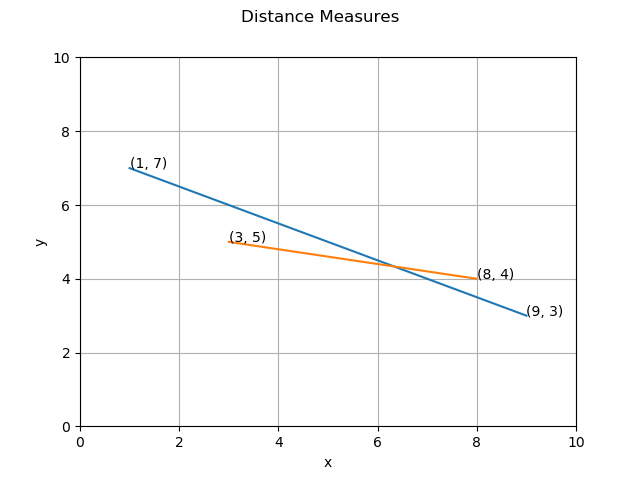
\includegraphics[width=.7\textwidth]{image/general/distance.png}
\caption{Example of Distance Measure}
\label{fig:distanceMeasure}
\end{figure}





\subsection{Color Model}

While humans' visible spectrum $(400nm - 700nm)$ can be represented using the respective wavelengths,  in order to describe these values in a 

\cc{to fill up... talk about color space and why}
%http://markkness.net/colorpy/ColorPy.html

\begin{figure}[hbt!]\centering
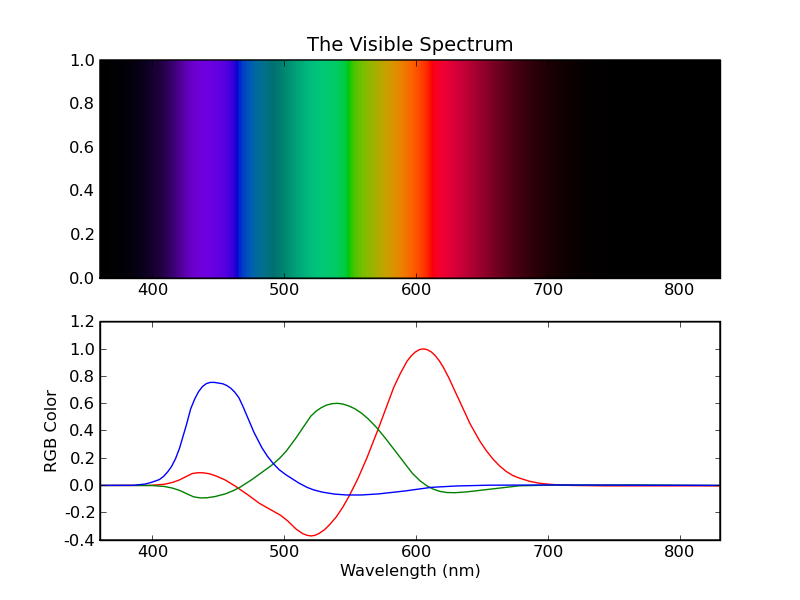
\includegraphics[width=.7\textwidth]{image/general/VisibleSpectrum.png}
\caption{RGB Values and their corresponding spectrum}
\label{fig:visibleSpectrum}
\end{figure}


\section{Framework Overview}
\label{section:framework}
In this section, a high level overview of the fundamental processing step along with two suggested core components for vehicle semantic extraction and retrieval is provided. The groundwork described in this work abides to the typical top-down approach used in Intelligent Transportation System (ITS) where the video data is subjected to background subtraction, followed by blob filtering, vehicle detection as well as vehicle tracking is as described in \cite{lim2017}. The semantic information from the vehicle blobs are then extracted and stored in the database. 

Now, with the vehicle specific semantics stored in the database, retrieval engines were designed to enabled users to easily retrieve the stored information. Both retrieval engines features a graphical user interface which allows users to enter the queries by drawing the desired trajectory on the search interface as well as providing other crucial information which would assist in identifying the targeted video shot.


\begin{figure}[hbt!]\centering
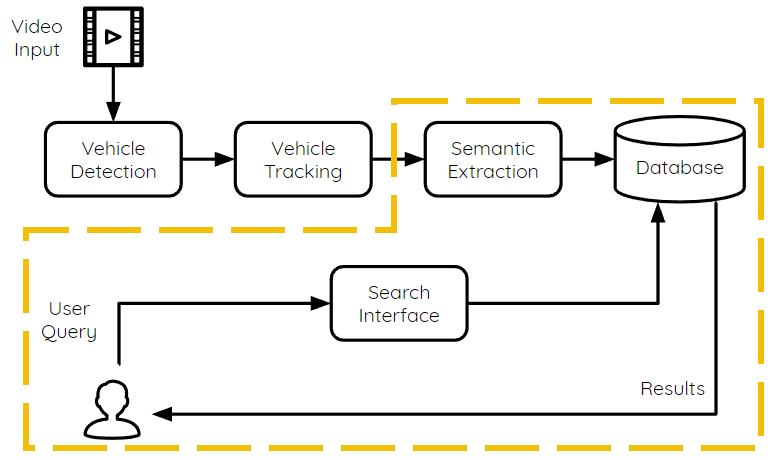
\includegraphics[width=.9\textwidth]{image/framework_new.PNG}
\caption{Framework Diagram, Contribution in Highlighted Border}
\label{fig:framework}
\end{figure}


In this work, two frameworks were suggested and used for the vehicle semantic extraction and retrieval process. Both frameworks utilize an underlying distinctive approach, with the same end goal in mind, which is the retrieval of desired video snippets which closely resembles a user described query. For each of these frameworks, the formulation of idea, steps and process involved are described in this chapter. 
%As there are various solutions proposed in this work, solutions which are common to both core frameworks is also provided. 
As a whole, the end-to-end framework can be visualized using Figure \ref{fig:framework} where the main contribution of this work is highlighted in yellow border. 

\subsection{LSH-Inspired Retrieval Framework}
The first of the two frameworks suggested in this work is the \textit{LSH-Inspired Retrieval Framework}. Locality-Sensitve Hashing (LSH) is a technique used for dimensionality reduction, typically to perform hashing on a set of documents so that documents with similar properties are mapped and clustered to similar locality or neighbourhood. This technique excels especially when working with high dimensional data such as video data.

Inspirations to cluster similar documents were drawn from the LSH technique and implemented in this framework. The extracted semantics from each vehicle blobs were clustered into semantic groups which contains color and motion information. This concept was adopted in the proposed method with the following considerations in mind: 

\begin{enumerate}
    \item Ease of Interpretation \& Access: As the extracted semantics are stored in clusters of similar properties, these semantics can be easily interpreted and retrieved. 
    \item Reduction of Input/Output (I/O) Bottleneck: As the proposed method stores the extracted semantics in a database, I/O bottlenecks are bound to occur when reading and retrieving large quantity of data. As the semantics of similar properties are clustered together, the retrieval engine does not have to search through the entire set of database for records that matches the given query.
\end{enumerate}


\subsection{Chamfer Distance-Inspired Framework}
The second of the two frameworks suggested in this work is the \textit{Chamfer Distance-Inspired Framework}. Chamfer distance is one of the many distance measure (see Section \ref{section:distancemeasures}) introduced by mathematicians and researchers. Chamfer Distance, as introduced by \cite{barrow1977parametric}, was originally designed to match images by comparing the shapes of two collections of shape fragments. However, in this framework, the use of chamfer distance was modified to suite the research problem of comparing the shapes of vehicle trajectories. While the implementation of chamfer distance measure in this framework has its advantages, it also comes with some drawbacks. The considerations taken when designing this frameworks are as such:


\begin{enumerate}
    \item The use of Chamfer Distance to compare trajectories allows the retrieval engine to search from a wider range, however, this comes with extra computational cost. While the disadvantages were undesirable, the benefits outweighs this drawback by providing a higher recall rate for the retrieved results. Along with that, the use of time and date filtering could potentially reduce the number of records, hence, further reducing the computational cost. 
    \item The ranking of results is a desirable feature in a retrieval engine. As Chamfer Distance produces a distance score for every pair of trajectories compared, this score can be used to sort the results in an intuitive manner where results of higher resemblance would appear higher in the ranking.  
\end{enumerate}


\section{Dataset}
\label{section:dataset_used}

In view of testing the proposed framework for large-scale extraction and retrieval of video semantics, a new collection of video dataset was gathered. A stationary cloud-enabled web camera was set up on the fourth floor of a building with a window facing a piece of private car park area. Figure \ref{fig:camerasetup} depicts the camera setup overcasting the car park area. 

The aforementioned setup was done to mimic a typical camera setup which tower over a piece of outdoor car park lot that are found in the wild. 


\begin{figure}[hbt!]\centering
\includegraphics[width=.8\textwidth]{image/fcicar park2.png}
\caption{Camera setup to capture the car park from the fourth floor}
\label{fig:camerasetup}
\end{figure}


\begin{figure}[!hbt]\centering
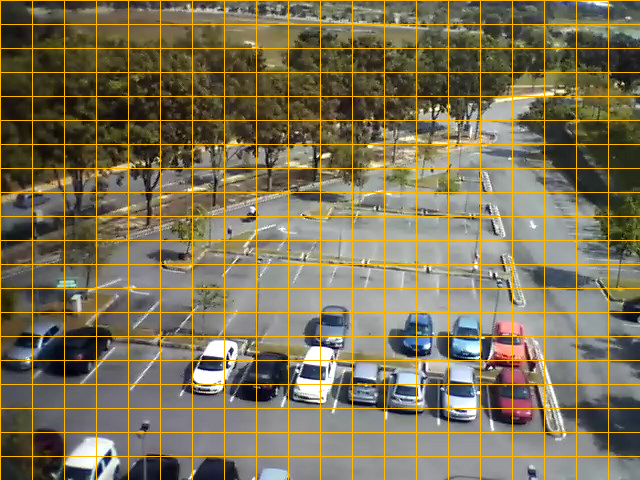
\includegraphics[width=.7\textwidth]{image/general/grids.png}
\caption{View from camera setup; 20$\times$20 Grids}
\label{fig:viewfromcamera}
\end{figure}


Through the camera's web interface, this device was set to record on weekdays from Monday through Friday, starting from 08:30 in the morning up until 18:30 in the evening, with a total of 10 hours of video being recorded each day. Among the important settings, each recorded video clip was set to have a maximum length of 6 minutes, and hence, 10 video clips every hour, and a total of 100 at the end of each day. The recorded video clips were saved into the external microSD memory card. At the end of each day, the data was then copied over to a server via a script. However, due to glitches that occurred during the recording process, some of the video clips were cut off abruptly. Hence, some of the days do not contain the full 10 hours video clips. 

\begin{table}[]\centering
\begin{tabular}{ll}
Camera Model: & Dlink DSC-942L        \\
Resolution:   & 640$\times$480 pixels \\
Frame rate:   & 10 $fps$             \\
Format:       & H.264 / MPEG-4 AVC    \\
Naming Convention: & $CCYYMMDD\_HHMMSS.mp4$
\end{tabular}
\vspace{1em}
\caption{Camera details}
\end{table}

\begin{figure}[htb!]
  \centering

\begin{tabular}{cc}
 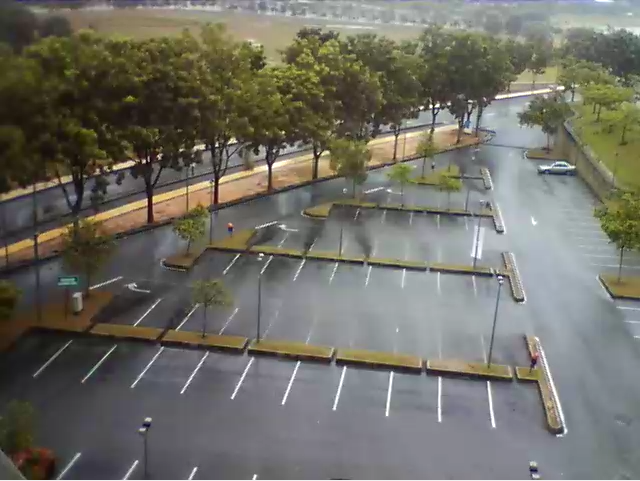
\includegraphics[width=0.4\linewidth]{image/general/rain.PNG} &  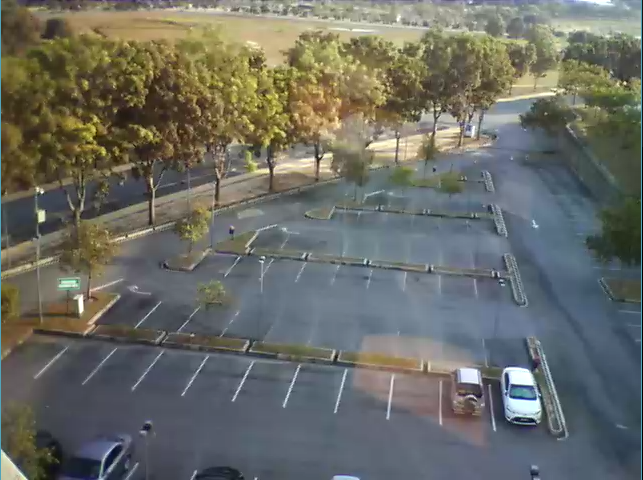
\includegraphics[width=0.4\linewidth]{image/general/reflection.PNG}\\ 
\begin{tabular}{c}(a) Rainy day with \\ reflective surface\end{tabular} & \begin{tabular}{c}(b) Reflection on the \\car park from the window\end{tabular} \\
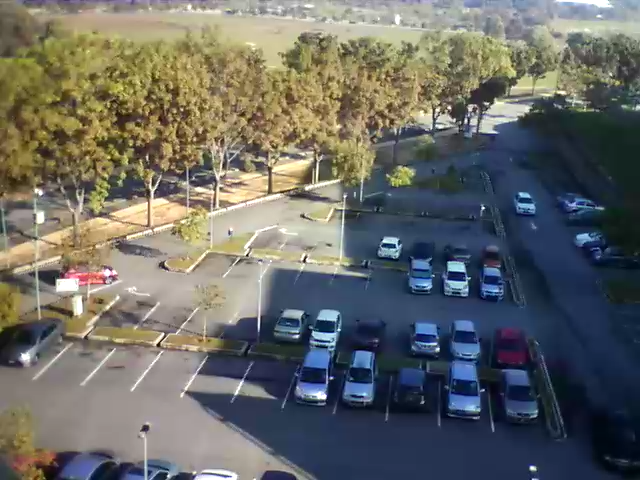
\includegraphics[width=0.4\linewidth]{image/general/shadow.png} &  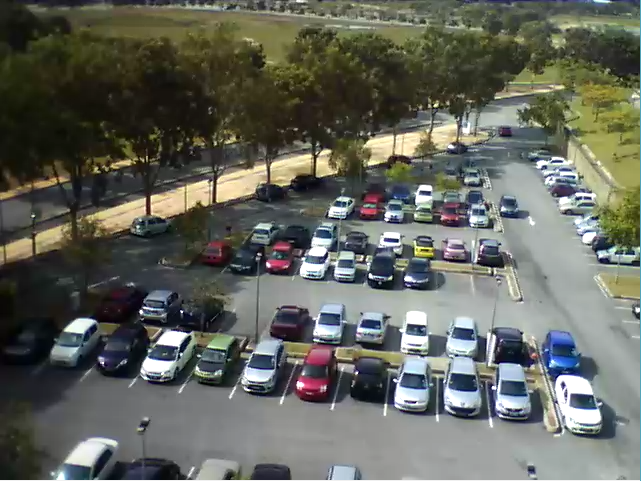
\includegraphics[width=0.4\linewidth]{image/general/shadow2.png}\\
\begin{tabular}{c}(c) Severe shadow over \\ the car park (08:48AM)\end{tabular} & \begin{tabular}{c}(d)  Severe shadow over \\ the car park (04:06PM)\end{tabular}
\end{tabular}


\caption{Noisy data within the collected dataset} \label{fig:weather}
\end{figure}


This setup was left to record data over the course of several months with various weather conditions, lighting conditions as well as a diverse set of car park scenes which includes peak hours with plenty of vehicles along with the off-days. In addition to that, this setup covers a total of over 45 parking lots which excludes parking lots that are too small or occluded. Figure \ref{fig:weather} exhibits the various weather conditions and noise which were recorded sporadically throughout the dataset.





\section{Experimental Methodology}
\label{sec:expmethodology}

In the subsequent chapters, the detailed descriptions of the proposed vehicle semantic extraction algorithm as well as the retrieval engine modules will be provided. In this section, the methodology and the experimental setup is briefly discussed to provide an overview on how the experiments will be performed in this work.

As the performance of the proposed method is essential towards end users, each of the proposed algorithm in the framework is evaluated with the help of volunteers. Even though the fundamental framework was adopted from \cite{lim2017} without changes on the underlying algorithm, errors which were propagated from the Vehicle Detection and Vehicle Tracking modules were not overlooked nor discarded during the evaluation of the subsequent modules in the pipeline. This was done intentionally to provide an end-to-end assessment of the framework. 

The proposed methods were implemented and evaluated on an Intel i7 machine with 16GB RAM, GeForce GTX 1060 GPU. As the main focal point in this proposed method revolves around the semantic extraction of vehicle color along with the vehicle trajectory, both of these components were assessed and evaluated individually to better understand the performance, effectiveness as well as the weakness of the proposed methods. This, in turn, provides a deeper understanding and opportunities for improvements as well as future works. 

While the collected dataset comprised of several months of data, only two days of data were used for the evaluation of \versionOneRet. These data were  fully annotated manually by several annotators and cross-checked to arrive at a consensus. The  annotated dataset included the total number of vehicles with their corresponding color categories. The total number of vehicles performing $TQ1$ \& $TQ2$ (see Figure \ref{fig:versionOneInterface}).


However, as with any retrieval engine for all intents and purposes dealing with long-term data, it is not feasible to annotate a huge amount of ground truth manually as it is a labour intensive, mundane and time consuming process. Hence in the \versionTwoRet, one month of data was processed and evaluated without the manual annotations of all the events. 
%Instead, the best practice used in evaluating a large scale retrieval engine was used to document the evaluation process. 
Instead, this evaluation process took on an empirical user study approach. Here, a group of six volunteers were tasked to perform queries on the retrieval system and provide relevance score for each retrieved results. 

%Justify why the experimental methodology for both frameworks are different
\cc{hmm not sure how to justify why different experimental methodology was used for these frameworks}


